\documentclass{article}
\usepackage[utf8]{inputenc}
\usepackage[margin=0.75in]{geometry}
\usepackage{sectsty}
\sectionfont{\fontsize{14}{15}\selectfont}
\usepackage{graphicx}
\usepackage{subcaption}
\usepackage{amsmath}
\DeclareMathOperator{\sign}{sign}
\usepackage{amssymb}
\usepackage{float}
\usepackage{enumitem}
\usepackage{stmaryrd}
\usepackage{textcomp}
\usepackage{booktabs}
\usepackage{appendix}
\title{MLTech Final Project}
\author{Ching-Yuan Bai, Hai-Tao Wu, Sheng-Fu Wu}
\begin{document}
\maketitle

\section{Initial Ideas}
The competition is a regression problem where the goal is given the background knowledge of users and books, predict the rating of user-book pairs. The first thing we noticed is that there are two separate tracks, 1 and 2. Track 1 uses mean absolute error as evaluation cost function and track 2 uses mean absolute percentage error which penalizes lower score groups more which implies using same models for track 1 (by simply rounding off to whole numbers) and 2 may not yield best results.

We also observed that features generally require being process before actual usage since the dataset is quite unorganized and contains significant amount of missing values as well as non-uniformity in format of data. Due to the size of incomplete data, we are unable to simply discard them and use the remaining for training. Thus methods should be developed to extract relevant information from the originally information-sparse dataset. Some of the missing values are hard to be compensated, such as locations and ages of users, which leads to issue of choosing which features to remove entirely. 


Some basic statistical analysis shows that for all the users and books information provided, there exists immense difference in information richness regarding each instance. 
% Give a brief insight of how great the disparity is between data
% insert the graph of distribution between books and users
Because of the high dimensionality of features and asymmetric distribution between books and users, we need to summarize the data first with methods like squeezing, auto-encoding, and matrix factorization.


Statistical analysis also shows that most of the users ratings are concentrated around 7 and 8. Thus we can expect that most of the models trained are highly likely to predict ratings concentrated in such region and a failed model is probably will always output rating of constant 8 for every instance, providing first-line evaluation of model performance aside from testing error.

\section{Preprocessing}
% More technical detail regarding the actual implementation of preprocessing.

Preprocessing data to usable format goes a long way in training a successful model. Due to the property of the dataset, having attributes that generally require some kind of treatment to actual utilize, we came up with several procedures to modify the dataset.


\subsection*{Missing values}
Regarding the missing values, we filled in the median of the feature and added another feature, \texttt{isNA} to record whether the value is artificially added or not. The \texttt{isNA} can be useful to prevent bias towards the median when applying linear models. For decision tree models it may be more useful than the original value if the people with same missing values have certain similar property. For example, it is possible that elderly people are less skillful at using electronic devices thus may be more likely to leave the age label empty. In this case, using the \texttt{isNA} feature might be more useful than the age value if the tree is trying to separate data relating to the users' age.
% some technical details to be filled here
% how to fill in the missing value for what and why do so instead of others

\subsection*{Feature extraction}
We are given the location of the user in the users data, which does not contain much information in the string of country names or city names. However, we can clearly see that geographic constraints may be an influential factor on the ratings of a book. People in similar regions may have more aligned values and taste for books. For example, suppose the book is about Christianity, then it may be more likely to obtain higher ratings from users from western countries. Thus we transformed the location names into actual coordinates in terms of latitudes and longitudes, which can exactly represent the distance of regions in numerical values. By doing so, it is possible to obtain continuous similarity for location of users, rather than discrete categorical features and making it easier to apply to models.


On the other hand, ISBN is a 10 or 13 digit of number with little to none meaning numerical-wise. It consists of information regarding the group, publisher, and the title of a book. In fact the last digit is a check-sum so should provide no extra information. Similar to transforming location name to geographical coordinates, we decided to represent the most obvious feature provided by the ISBN, the group (nationality), as a categorical feature extract more specific knowledge in compound feature as ISBN and discard the useless checksum to reduce noise.


\subsection*{Encoding}

Since the book and user data contains a wide range of information size difference, with some users having ratings for 13602 books, while others may not have any record or only implicit ratings. As for the books, some may receive enough ratings where the distribution of ratings can truly reflect its future ratings while most of the others have only less than one rating and some may be never rated before. A method to organize the diverse and chaotic data is required, and our take on it is by auto-encoding and statistical analysis due to the many missing values, which would be hard to unify without some statistical representative index.

We choose the following indexes to summarize users and books data, number of instances, quantile (11 bins), mean, mode, standard deviation, skew, and kurtosis. Specifically choosing kurtosis while simultaneously choosing standard deviation may be able to emphasize on extreme values. Number of instances is also an important factor which can determine if a book is a bestseller (which may likely result in generally higher ratings).

For auto-encoder we encode the features for a book by first one-hot encoding all of the users that have read this book before, with all users including users in training, implicit, and testing set. Thus this is an offline learning schema. Then we remove the users that have only read 200 or less books so what remains are users that have a record of reading 200 or more books. The reasoning behind this action is because we can assume that people who have read more books can represent behavior of other people who have not read that many books. Then we auto-encode the (200,1) one-hot vector and add it into the feature of a book. Same can be done for users, where we choose books that have received 400 or more ratings as qualified candidates and add the auto-encoded features into each book.

\section{Models}

% introduce the approaches tried! (maybe failed)
% Don't compare models yet.

% Sketch of how to describe each model
% 1. Why choose this model for this problem? What is its specialty that it is chosen over other models?
% 2. What is the expected result, because not all models are all used for training for the final prediction (ex. lasso for feature selection)? How can it achieve that goal? (some properties of this particular model)
% 3. Technical details regarding how the model is used but exclude performance, including which package, what parameters is tuned, etc.
% Goal is #replicability!!!!!!!!!!!!!!!!!!!

\subsection{Linear Model}
For the linear model, we define
% For the linear model, first we separated an subset of the original training set to use for validation and will be naming the error calculated by this separated set as $E_\text{test}$ in future mentions. Then we define the model as
$$
{y_i}_\text{predict} = a_1 \hat{U_i} + a_2 \hat{B_i} + a_3, \quad \text{with conditional } a_4, a_5
$$
where for each book-user rating pair $\{(u_i, b_i)\}_{i=1}^N$, we can obtain $\hat{B_i}$ the average rating of the book $b_i$ and $\hat{U_i}$ the average rating user $u_i$ gives, determined from the training set. If the book have never been rated before then it is given the constant $a_4$ to replace $\hat{B_i}$ and same for the user, where when the user have never rated any book then $a_5$ is used to replace $\hat{U_i}$. Thus the error for track 1 and track 2 is simply
$$
E_\text{MAE} = \frac{1}{N} \sum_{i=1}^N |{y_i}_\text{predict} - y_i|
, \quad
E_\text{MAPE} = \frac{1}{N} \sum_{i=1}^N \frac{|{y_i}_\text{predict} - y_i|}{y_i}
$$
respectively, and we choose to optimize the error by simulated annealing. The reasoning behind using simulated annealing is mainly due to the large number of missing values in dataset. When the validation set consists of a great percentage of missing values, the remaining effective data to determine optimal parameters reduces, which results in higher probability to overfit the validation set. Thus cross validation is necessary to tune parameters $a_1 \cdots a_5$ in order to prevent such situations, where the training half is used to calculate $\hat{U}$ and $\hat{B}$ and the validation half determines the performance $E_\text{val}$. However, we are unable to find machine learning packages that support MAE and MAPE (inverse/pseudo-inverse matrix optimizes MSE) with cross validation. On the other hand, simulated annealing isn't based on any prior assumptions of the target function and dataset and tries to find global minimum, which perfectly applies to the problem we wish to solve. Some details regarding the linear model is listed below:
\begin{itemize}
\item Initial temperature for annealing is fixed at 15\textdegree
\item $a_1, a_2 \in [-0.2, 1.2], a_3 \in [-2, 2], a_4, a_5 \in [4, 10]$
\item 24-fold cross validation each with 120000 iterations of linear cooling
\end{itemize}
\subsection{Gradient Boosting Decision Tree}
% parameter selection: many shallow trees vs little deep tress, learning rate
Tree models have the benefits of high efficiency and great interpretability with results aligned with human intuition. It also won't be affected by the numerical range of features, thus normalization or rescaling is unnecessary. We choose to use the Microsoft project, Lightbgm to implement the model. They main reason choosing LGBM over traditional XGBM is due to how these models are regularized. XGBM is mainly regularized by setting the maximum number of layers so the trees are mostly symmetric and full while LGBM is mainly regularized by limiting the total number of leaves for each tree, thus the shape can differ for each tree increasing diversity for boosting. LGBM is prevented from overfitting by the numerous regulation parameters resulting the dichotomies not being shattered entirely and thereby controls VC dimension of the model.


One interesting phenomenon we observed is of all the best performing models, some consists of many shallow trees while others consists of small number of deep trees. Intuitively, we can either increase the depth of each tree or increase the total numbers of trees in order to achieve the required complexity to match the dataset, despite the underlying different physical meaning. Another phenomenon we observed is when the training set is sufficiently large in terms of size, we can increase the \texttt{min child samples} (to form new node) parameter, which effectively increases the efficiency of branching.


In general gradient boosting tree packages, there are many customizable parameters. But many parameters have similar effects, for example, limiting the number of leaves somewhat bounds the max depth of a tree. Thus the parameters we choose to tune are \texttt{number of leaves}, \texttt{min child samples} (to form new node), \texttt{learning rate}, and \texttt{n estimators} (maximum number of trees allowed to grow). Since each iteration of training is extremely efficient, we are able to properly tune the chosen parameters to achieve optimal performance for LGBM.


\subsection{Deep Neural Network}
Deep neural network, representing the most popular model in current machine learning world, claiming to be able to optimize basically most of the problems, is chosen as one of our models to experiment on. Due to the constraint of computing power and computation time, we picked two models, SeLU and ReLU + batch-norm to further investigate their performance on the dataset. These two methods are chosen because first of all they are the most popular models that can deal with obvious weakness of DNN in recent years, and secondly we expect the gradient of each layer may differ in multiple orders of magnitudes of due to inhomogeneity of meaning for each feature.


There are a huge number of parameters that can be tuned in a deep neural network, but again, due to limitation of computing power and computation time we choose the three most important parameters, learning rate, depth of network, and the number of nodes in each layer. Here we let all layers have same number of nodes with same activation function for simplicity and solve with ADAM. For each combination of parameters, we run for 30 epochs or for 900 seconds, depending on which threshold is reached first and choose the best performing epoch for $E_\text{val}$. In each epoch data is split into mini batches of size 1024.
To be more efficient in parameter tuning, we proposed an interesting schema which strictly outperforms random search and can yield interesting insight regarding the model which we will discuss later.

\subsubsection*{Self-Normalizing Neural Networks}
SeLU is a modified version of eLU where the generated output is more stable compared with other activations. The original paper with more than a hundred pages of proof claims that by applying the LeCun normalization for initializing the weights and using the scaled activation, the output gradually approaches N(0,1) which will prevent extreme values of gradients thus allowing larger learning rate to be applied. The acceptable learning rate can be as large as 0.08 in our experiments, greatly reducing the possibility of failure in training some combinations of parameters. Since both SeLU and batch-norm attempts to let the output approach $N(0,1)$, it is generally both redundant and not efficient to apply both methods together.

% require enough layers to achieve self normalization by SELU
\subsubsection*{Batch Normalization}
Batch normalization is a method proposed before SeLU but widely used combined with ReLU to stabilize output values. Some slight differences when compared with SeLU is that while SeLU lets the output approach $N(0,1)$ over iterations, batch norm attempts to stabilize output by first normalizing the mini-batch then adding free parameters to return the deprived degree of freedoms. The acceptable learning rate can be as large as 0.6 in our experiments, robustly safeguarding the gradient from exploding under high learning rates.

\subsubsection*{Optimized random search}
In order to increase the efficiency of tuning parameters, we proposed a method to improve the naive random search adopted in general cases. When choosing an combination of parameters to optimize, we face the exploration-exploitation dilemma where on one hand we wish to explore combinations far away from points already explored in order to try for even better performance, but on the other hand we also wish to select points closer to good-performing parameters explored in the past, exploiting the fact that neighboring points should perform similarly well as well. 


We can define the value for utility gained by exploring as $\sigma(x)$ and utility gained from exploitation of previous good points as $\mu(x)$. The function $\sigma(x)$ is determined by L1-norm to the closest neighbor and $\mu(x)$ is determined by averaging KNN performance of past queried points on the parameter space.

Suppose we sample $N$ candidates of parameter combinations $S = \{p_i\}_{i=1}^N$ each with the expected utility gained from exploration and exploitation of $\sigma(p_i)$ and $\mu(p_i)$ respectively. Then we can further reduce the candidate such that remaining members has $\sigma$ and $\mu$ not being strictly dominated, i.e. there exists no other candidate that has both a higher $\sigma$ and $\mu$. By empirical observations, the remaining candidate set, denoted as $S^*$ consists of approximately 10 members, despite the number of candidates $N$ originally sampled. Thus $S^*$ forms a efficiency frontier where the max gain can happen for the next query when parameters are selected from $S^*$.

\begin{figure}[h]
\begin{subfigure}{.5\textwidth}
  	\centering
  	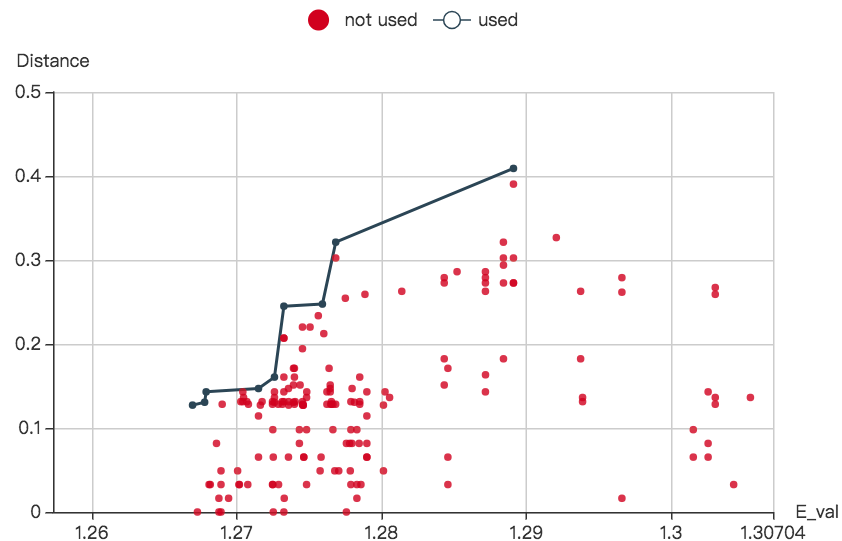
\includegraphics[width=.8\linewidth]{frontier.png}
  	\caption{Visualize efficiency frontier}
\end{subfigure}
\begin{subfigure}{.5\textwidth}
  	\centering
  	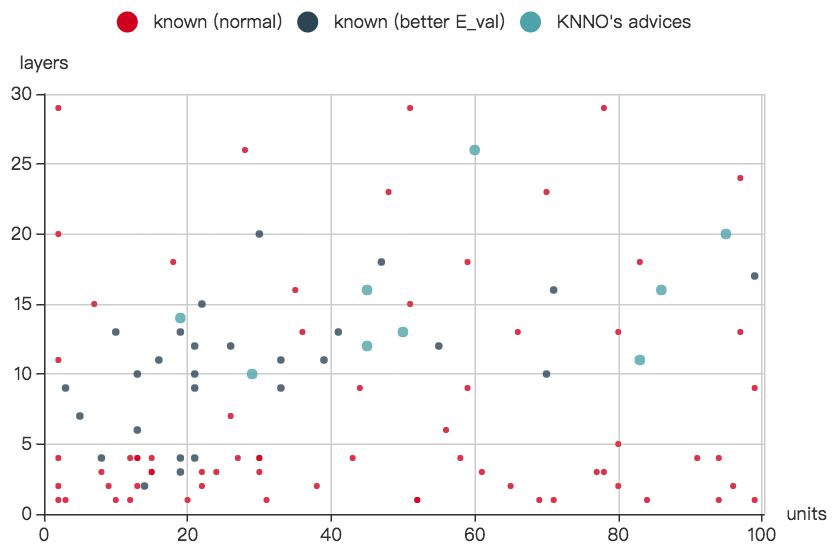
\includegraphics[width=.8\linewidth]{knno.png}
  	\caption{Visualize suggestion by optimized random search}
\end{subfigure}
\end{figure}

Multi-threading can be applied when partitioning the frontier to multiple sections with difference preference of exploration / exploitation. Ideally all of the threads have to be finished and synced before the next round of frontier can be determined. However, in order to further accelerate calculation, we implemented the multi-threading by splitting into two threads with one processing the half of frontier where it prefers exploration while the other explores the half of frontier where it prefers exploitation. Then we can synchronize the two threads after multiple iterations since both threads are expected to choose drastically different (independent) parameters to search.



\subsection{Matrix Factorization}
At first glance, matrix factorization seemed likely the perfect solution to the user-book rating prediction problem. If we consider a matrix with users as columns and books as rows, the $(i,j)$ element then represents the rating the $i$-th user gives the $j$-th book. Given some of the values of the matrix, we have to solve for other missing elements, exactly what matrix factorization is made to do. We apply simple gradient descent to optimize and apply validation to tune for the dimension of U and V, the two factorized matrices. L2 regularization is added to prevent overfitting due to the underlying nature of neural networks.

As ideal as it seems, both the information regarding the user and the book are required in order to predict properly. However, in the given testing set, a significant portion of book or user have never existed in past training data before, which would require augmented data from other models to fill in the gap. Small size of features regarding each book and user may also degrade the performance of prediction. Thus it can be expected that matrix factorization may not be the best-performing model. 

\begin{table}[ht]
\begin{minipage}[b]{.45\textwidth}
\centering
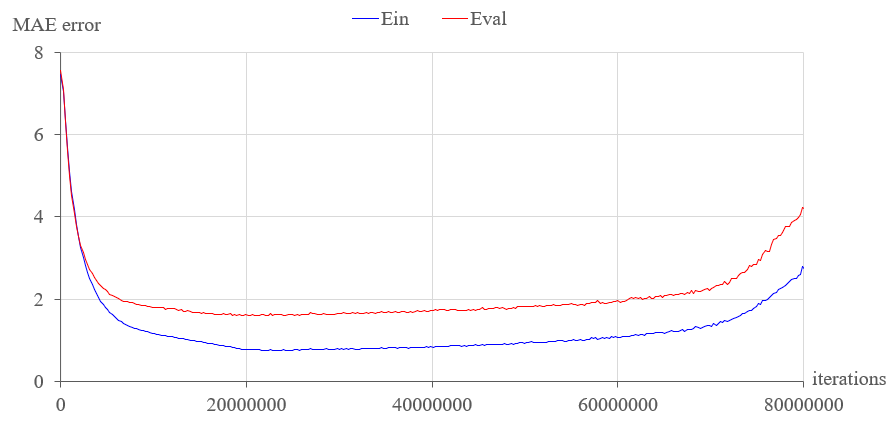
\includegraphics[width=\linewidth]{mf_error_vs_iter.png}\\
(a) MF: Loss vs Iterations
\end{minipage}
\begin{minipage}[b]{.55\textwidth}
\setlength{\tabcolsep}{3pt}
\centering \footnotesize
\begin{tabular}{r|llllllllll}
&\multicolumn{10}{c}{Track 2}\\
%\cline{2-11}
Track 1&1&2&3&4&5&6&7&8&9&10 \\
\midrule
1&0&0&0&0&0&0&0&0&0&0\\
2&0&0&0&0&0&0&0&0&0&0\\
3&0&0&0&2&0&0&0&0&0&0\\
4&0&1&5&100&32&2&0&0&0&0\\
5&0&0&10&185&4766&1281&5&0&0&0\\
6&0&0&47&249&1095&8669&1231&14&0&0\\
7&0&0&0&8&226&5940&29245&2281&10&0\\
8&0&0&0&0&0&67&30234&50442&3092&0\\
9&0&0&0&0&0&0&9&9280&15777&151\\
10&0&0&0&0&0&0&0&0&6824&2189\\
\bottomrule
\end{tabular}\\
\normalsize



(b) Prediction of test set by best model of track1 / track2 \\
(Track 2 generally predicts lower ratings than track 1)
\end{minipage}
\end{table}

\subsection{Ensemble}
For all the previous models, we did a simple weighted-mean or weighted-average ensemble to blend them together. Since it is expected that every model has specific points that it performs unusually terrible, by taking the median/mean of each model weighted by $\frac{1}{s_m-a}$ (where $s_m$ is the public score for the model and $a$ is a constant), we can select the relatively conservative and mediocre answer, which is less likely to be erroneous.

\subsubsection*{Blending for Track 2}
Since track 2 penalizes errors in lower score regions more, we proposed an specially designed blending the incorporate the unique characteristic. For the blending model proposed above, because it can be weighted by public scores in MAE and MAPE, we can obtain two sets of predicted ratings. For each instance, we select the \textbf{minimum} of the two sets. This can be intuitively explained since if a rating is low given by MAE, then the rating  should be even lower given MAPE, for MAPE is naturally biased towards the lower end of the rating spectrum.

\section{Performance and Discussion}

\begin{table}[ht]
\captionof{table}{Performance of models for track 1}
\centering
\begin{tabular}{lllll}
	\toprule
    & Public Score & Private Score & Optimal Parameters & \\
    \midrule
    Linear & 1.256989 & 1.247220 & $(a_1,a_2,a_3,a_4,a_5)=(0.969,0.147,-0.7,7.736,6.524)$ \\
	LightGBM & 1.239182 & 1.233948 & \begin{tabular}{@{}c@{}}num\_leaves: 151, learning\_rate: 0.042625, \\ n\_estimators: 295, min\_child\_samples: 61 \end{tabular} \\
	SELU & 1.254969 & 1.252043 & units: 81, layers: 12, learning\_rate: 0.006571 \\
	BatchNorm & 1.250857 & 1.246115 & units: 47, layers: 18, learning\_rate: 0.071708 & \\
    MF & 1.371927 & 1.364194 & \begin{tabular}{@{}l@{}} dimension: 55, learning rate: 0.03 \\ C: 0.02, iterations: $7.8\times 10^ 7$\end{tabular} \\
    Ensemble & 1.216525 & 1.210063 & weighted average \\
	\bottomrule
\end{tabular}
\end{table}

\begin{table}[ht]
\captionof{table}{Performance of models for track 2}
\centering
\begin{tabular}{lllll}
	\toprule
    & Public Score & Private Score & Optimal Parameters & \\
    \midrule
    Linear & 22.157879 & 21.761054 & $(a_1,a_2,a_3,a_4,a_5)=(0.898,0.32,-1.857,7.477,6.683)$ \\
	LightGBM* & 22.792332 & 22.501919 & \begin{tabular}{@{}c@{}}num\_leaves: 151, learning\_rate: 0.042625, \\ n\_estimators: 295, min\_child\_samples: 61 \end{tabular} \\
	SELU* & 23.420125 & 23.185040 & units: 81, layers: 12, learning\_rate: 0.006571 \\
	BatchNorm* & 22.341601 & 22.076369 & units: 47, layers: 18, learning\_rate: 0.071708 & \\
    MF & 23.803070 & 23.394816 & \begin{tabular}{@{}l@{}} dimension: 45, learning rate: 0.03, \\ C: 0.025, iterations: $3.9\times 10^ 8$ \end{tabular} \\
    Ensemble & 21.955054 & 21.595748 & weighted average \\
    Ensemble (track 2) & 21.763355 & 21.381223 & $\min(\text{track1, track2})$ \\
	\bottomrule
    \multicolumn{4}{l}{*Trained for MAE}
\end{tabular}
\end{table}

\noindent
Given identical tuned parameters, \texttt{BatchNorm} performs slightly better than \texttt{SeLU}. Given same time period for training \texttt{DNN} and \texttt{LGBM}, since \texttt{LGBM} trains significantly faster than \texttt{DNN} (an epoch for \texttt{DNN} generally takes approximately 30 minutes), \texttt{LGBM} is able to outperform \texttt{DNN}. \texttt{Ensemble (track 2)} performs exceptionally well for track 2, claiming second place on the scoreboard.

\begin{table}[ht]
\captionof{table}{Pros and Cons of Models}
\centering
\begin{tabular}{lllll}
	\toprule
    & Pros & Cons & \\
    \midrule
    Linear & Can optimize for any error function & \begin{tabular}{@{}l@{}} Complicated dataset may require unreasonably \\ low annealing rate \end{tabular} \\
	LightGBM & Most intuitive to human perception & Potentially overfit if not regularized properly \\
	DNN & Automatic extraction of implicit features & Time and power consuming training process \\
    MF & \begin{tabular}{@{}l@{}} Designed exactly for solving problems with \\ abstract features \end{tabular} & Unable to utilize additional features \\
	\bottomrule \\
\end{tabular}
\end{table}

\begin{table}[ht]
\captionof{table}{Comparison of Models}
\centering
\begin{tabular}{lllll}
	\toprule
    Property & Ranking & Explanation \\
    \midrule
    Efficiency & Linear $>$ LGBM $>$ MF $>$ DNN \\
	Scalability & DNN $>$ LGBM ? MF $>$ Linear & Transfer learning can be applied to DNN if large dataset \\
	Popularity & DNN $\approx$ LGBM $>$ Linear $>$ MF \\
	Interpretability & Linear $\geq$ LGBM $>$ DNN $\approx$ MF \\
	\bottomrule \\
\end{tabular}
\end{table}

\subsection*{Optimal model selection}
% Must recommend the BEST ONE for EACH TRACK
We suggest \texttt{weighted-average blending} for track 1 since it performs best regarding MAE, due to democracy in blending, reducing extreme erroneous value in each single model. We suggest \texttt{ensemble (track 2)} for track 2 since it yields optimal performance regarding MAPE, due to unique blending method that is able to exploit the preference of low ratings in track 2. It is worth noting that if the ratings is rounded for track 2 (even though it accepts float as predictions), the score is able to improve by $0.2 \sim 0.4$. We infer that the reason is because all ratings must be an integer. Thus predictions with trailing decimals always will have an residual contributing to error increase.
% pros and cons for choosing each model
\section{Conclusion}
In the report, we experimented on four individual models and two methods for ensemble to tackle the user rating problem. Our main conclusion is parameter tuning is significantly more important than the model itself, as we observed when comparing \texttt{LGBM} with \texttt{DNN}. For \texttt{DNN} sufficient number of layers is essential for the network to fully express its property, such as the iterative normalization in \texttt{SeLU}. The optimized random search method we proposed performs extremely well in reality, selecting parameters to experiment that human intuition can follow and yielding insight regarding what the network is currently trying to optimize. Finally tree models are most robust against datasets with large portion of missing values, whereas model like matrix factorization (requiring some level of completeness in training data) significantly drops in performance.

\begin{thebibliography}{9}
\bibitem{latexcompanion} 
Ioffe, Surgey and Szegedy, Christian. 
\textit{Batch Normalization: Accelerating Deep Network Training by Reducing Internal Covariate Shift}. 
eprint arXiv:1502.03167, 2015.
 
\bibitem{einstein} 
Günter Klambauer, Thomas Unterthiner, Andreas Mayr, Sepp Hochreiter
\textit{Self-Normalizing Neural Networks}.
eprint arXiv:1706.02515, 2017.

\end{thebibliography}
\textbf{Workload Distribution}
\begin{table}[ht]
\begin{tabular}{lllll}
	\toprule
    Member & Workload \\
    \midrule
    % H.T. Lin (X
    H.T. Wu & Implementation of LGBM and DNN, establish structured tuning procedures\\
	C.Y. Bai & Implementation of DNN, report writing\\
    S.F. Wu & Implementation of linear model, MF, and ensemble\\
	\bottomrule
\end{tabular}
\end{table}
\end{document}
